% Copyright 2018 Beckman Coulter, Inc.
%
% Permission is hereby granted, free of charge, to any person
% obtaining a copy of this software and associated documentation files
% (the "Software"), to deal in the Software without restriction,
% including without limitation the rights to use, copy, modify, merge,
% publish, distribute, sublicense, and/or sell copies of the Software,
% and to permit persons to whom the Software is furnished to do so,
% subject to the following conditions:
%
% The above copyright notice and this permission notice shall be
% included in all copies or substantial portions of the Software.
%
% THE SOFTWARE IS PROVIDED "AS IS", WITHOUT WARRANTY OF ANY KIND,
% EXPRESS OR IMPLIED, INCLUDING BUT NOT LIMITED TO THE WARRANTIES OF
% MERCHANTABILITY, FITNESS FOR A PARTICULAR PURPOSE AND
% NONINFRINGEMENT. IN NO EVENT SHALL THE AUTHORS OR COPYRIGHT HOLDERS
% BE LIABLE FOR ANY CLAIM, DAMAGES OR OTHER LIABILITY, WHETHER IN AN
% ACTION OF CONTRACT, TORT OR OTHERWISE, ARISING FROM, OUT OF OR IN
% CONNECTION WITH THE SOFTWARE OR THE USE OR OTHER DEALINGS IN THE
% SOFTWARE.

\chapter {Event Manager}\label{chap:event-mgr}

\section {Introduction}

The event manager (\code{event-mgr}) is a gen-server that provides a
single dispatcher for events within the system. It buffers events and
dispatches them to the log handler and a collection of other event
handlers. If the log handler fails, the event manager logs events
directly to the console.

\section {Theory of Operation}

The event manager is a singleton process through which all events in
the system are routed. Any component may notify the event manager that
something has occurred by using \code{event-mgr:notify}. This model
is illustrated in Figure \ref{fig:event-mgr-flow}.

\begin{figure}
  \begin{center}
    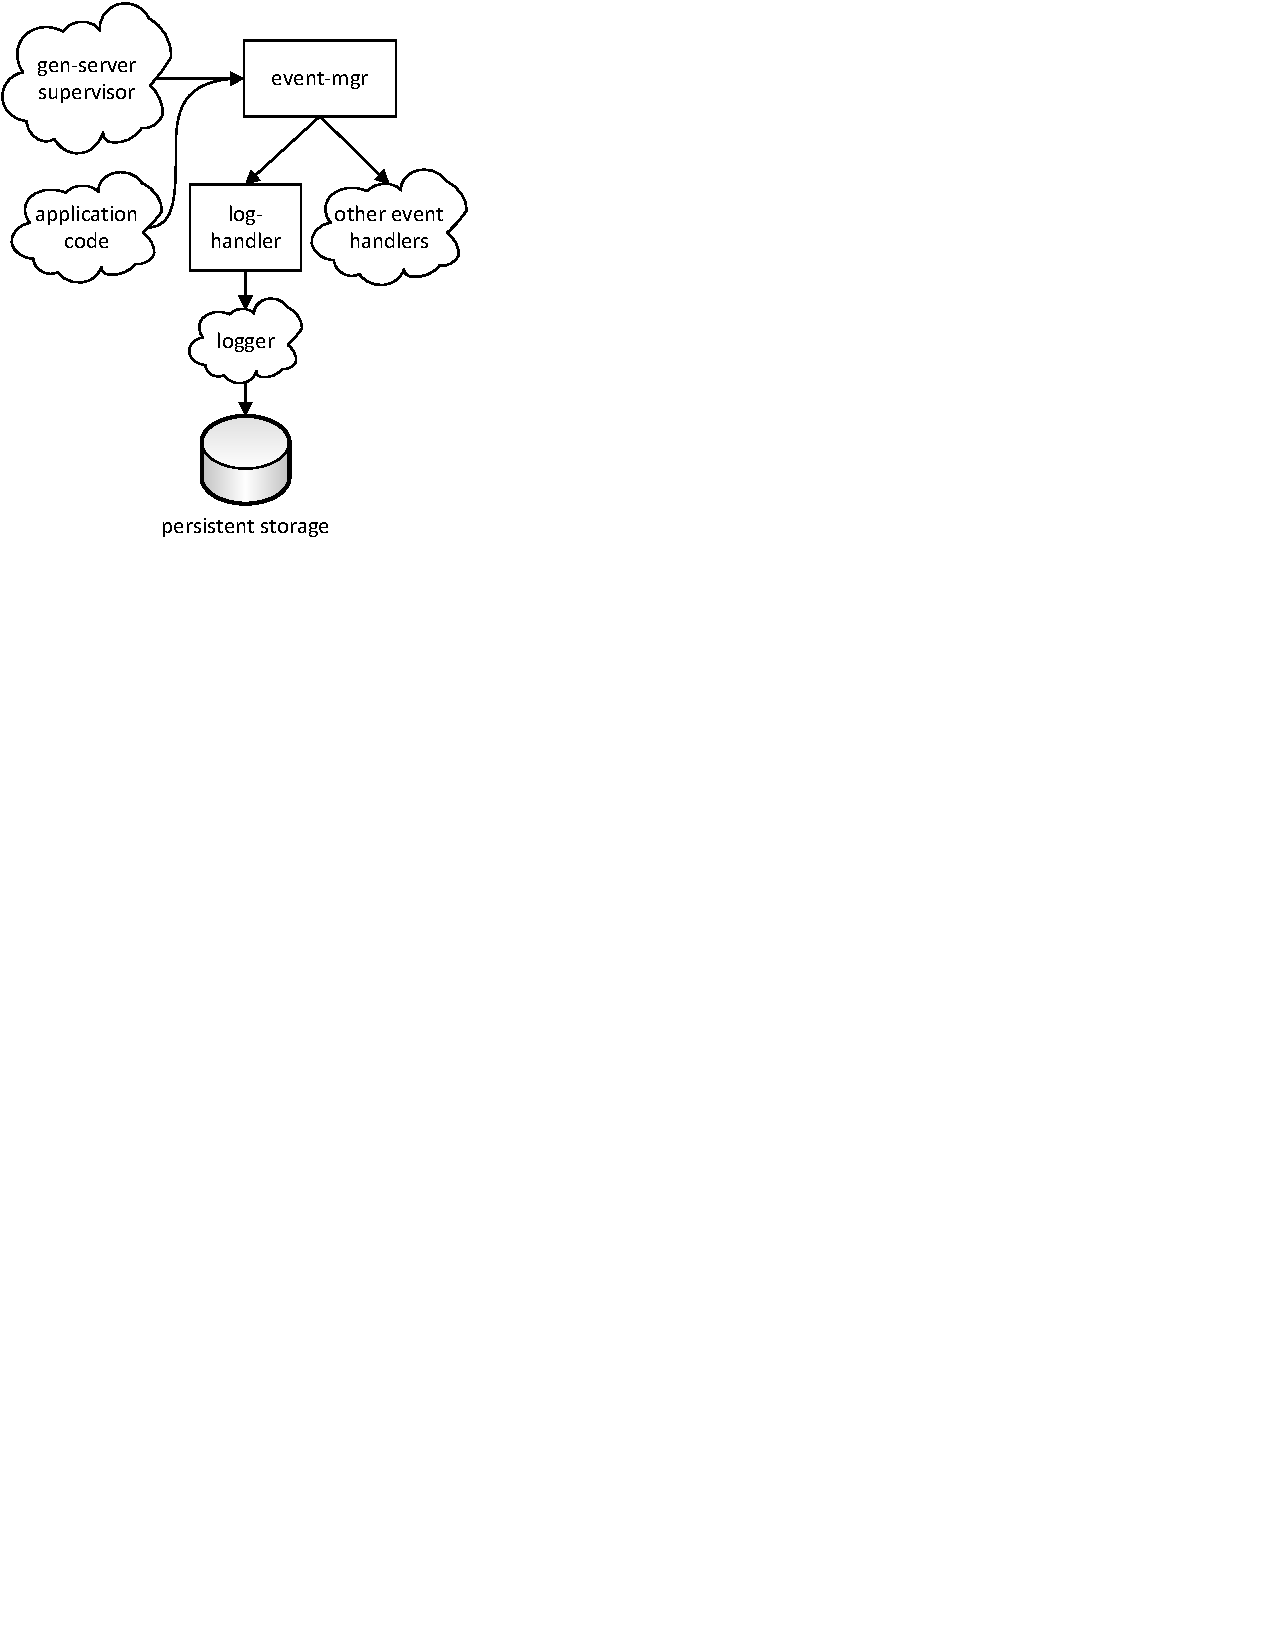
\includegraphics[trim=0 531 387 0]{swish/event-mgr-events.pdf}
  \end{center}
  \caption{\label{fig:event-mgr-flow}Event flow}
\end{figure}

The event manager is a registered process named \code{event-mgr}.

The event manager is created as part of the application's supervision
hierarchy. It buffers incoming events during startup until
\code{event-mgr:flush-buffer} is called. The buffered events are
then sent to the current event handlers and the log handler. This
provides the ability to log the startup details of processes,
including the event manager itself.

The event handlers should not perform blocking operations, because
they block the entire event manager.

If the log handler or its associated process fails, the event manager
logs events to the console. If another event handler fails with some
reason, the associated process is killed with the same reason. When
the process associated with a handler terminates, the event manager
removes it from the list.

\paragraph* {state}\index{event-mgr!state}
\begin{record}\code{<event-mgr-state>}\end{record}\antipar
\begin{argtbl}
  \argrow{event-buffer}{list of events to be processed (most recent
    first), or \code{\#f} when buffering is disabled}
  \argrow{log-handler}{\code{<handler>} record or \code{\#f}}
  \argrow{handlers}{list of \code{<handler>} records}
\end{argtbl}

\begin{recorddef}{<handler>}
  \argrow{proc}{procedure of one argument, the event}
  \argrow{owner}{process that owns the handler}
\end{recorddef}

\genserver{event-mgr}{init}The \code{init} procedure initializes the
state of the gen-server. Event buffering is enabled.

The gen-server traps exits so that it can detect failure of event
handler owner processes, as well as the \code{EXIT} message from the
parent process.

\genserver{event-mgr}{terminate}The \code{terminate} procedure
flushes any pending events to the console using \code{do-notify}.

\genserver{event-mgr}{handle-call}The \code{handle-call} procedure
processes the following messages:

\antipar\begin{itemize}

\item \code{\#(add-handler \var{proc} \var{owner})}: Link to the
  \var{owner} process, add a handler to the state and return
  \code{ok}.

  An invalid argument results in the following error reasons:
  \begin{itemize}
  \item \code{\#(invalid-procedure \var{proc})}
  \item \code{\#(invalid-owner \var{owner})}
  \end{itemize}

\item \code{flush-buffer}: Process the events in the buffer using
  \code{do-notify}, turn off buffering, and return \code{ok}.

\item \code{\#(set-log-handler \var{proc} \var{owner})}: Link to the
  \var{owner} process, set the log handler of the state, and return
  \code{ok}.

  An invalid argument results in the following error reasons:
  \begin{itemize}
  \item \code{log-handler-already-set}
  \item \code{\#(invalid-procedure \var{proc})}
  \item \code{\#(invalid-owner \var{owner})}
  \end{itemize}

\end{itemize}

\genserver{supervisor}{handle-cast} The \code{handle-cast} procedure
does not process any messages.

\genserver{event-mgr}{handle-info}The \code{handle-info} procedure
handles the following messages:

\antipar\begin{itemize}

\item \code{\#(notify \var{event})}: Process \var{event} using
  \code{do-notify}.

  \var{event} is any Scheme datum.

\item \code{\#(EXIT \var{pid} \var{\_})}: Removes the log or other
  event handler associated with \var{pid}.

\end{itemize}

Internally, the \code{(do-notify \var{event} \var{state})} procedure
handles the processing of each \var{event} with respect to the current
\var{state}. It evaluates the \var{state} in the following way:

\antipar
\begin{itemize}
  \item If the state is not buffering:
    \begin{enumerate}
    \item Call each handler's \var{proc} with \var{event}. If it exits
      for some reason, kill the handler's \var{owner} with the same
      reason.

    \item If there is a log handler, call its \var{proc} with
      \var{event}. If it exits for some reason, unlink its
      \var{owner}, kill it with the same reason, log \var{event} to
      the console using \code{console-event-handler}, and remove the
      log handler from the state.
    \end{enumerate}

  \item Otherwise, buffer the event.
\end{itemize}

\section {Programming Interface}

\defineentry{event-mgr:start\&link}
\begin{procedure}
  \code{(event-mgr:start\&link)}
\end{procedure}
\returns{}
\code{\#(ok \var{pid})} $|$
\code{\#(error \var{reason})}

The \code{event-mgr:start\&link} procedure creates a new
\code{event-mgr} gen-server using \code{gen-server:start\&link}.

The event manager is registered as \code{event-mgr}.

\defineentry{event-mgr:add-handler}
\begin{procedure}
  \code{(event-mgr:add-handler \var{proc} \opt{\var{owner}})}
\end{procedure}
\returns{} \code{ok} $|$ \code{\#(error \var{reason})}

The \code{event-mgr:add-handler} procedure calls
\code{(gen-server:call event-mgr \#(add-handler \var{proc}
  \var{owner}))}.

\var{proc} is a procedure of one argument, the event. Failure in
\var{proc} results in the event manager killing the \var{owner}
process with the same failure reason. The handler is removed when the
event manager receives an \code{EXIT} message from \var{owner}.

\var{owner} is a process. The default is the calling process.

\defineentry{event-mgr:flush-buffer}
\begin{procedure}
  \code{(event-mgr:flush-buffer)}
\end{procedure}
\returns{} \code{ok}

The \code{event-mgr:flush-buffer} procedure calls
\code{(gen-server:call event-mgr flush-buffer)}.

\defineentry{event-mgr:notify}
\begin{procedure}
  \code{(event-mgr:notify \var{event})}
\end{procedure}
\returns{} \code{ok}

The \code{event-mgr:notify} procedure sends message
\code{\#(notify \var{event})} to registered process
\code{event-mgr} if it exists. If \code{event-mgr} does not exist,
it prints \var{event} using
\code{console-event-handler}.

\var{event} is any Scheme datum.

Because the gen-server library uses \code{event-mgr:notify}, it is
implemented there.

\defineentry{event-mgr:set-log-handler}
\begin{procedure}
  \code{(event-mgr:set-log-handler \var{proc} \var{owner})}
\end{procedure}
\returns{} \code{ok} $|$ \code{\#(error \var{reason})}

The \code{event-mgr:set-log-handler} procedure calls
\code{(gen-server:call event-mgr \#(set-log-handler \var{proc}
  \var{owner}))}.

\var{proc} is a procedure of one argument, the event. Failure in
\var{proc} results in the event manager killing the \var{owner}
process with the same failure reason. The log handler is removed when
\var{proc} fails or the event manager receives an \code{EXIT}
message from \var{owner}.

\var{owner} is a process.
